% LAB 12: Project
%
% CSE/IT 107: Introduction to Programming
% New Mexico Tech
%
% Prepared by Russell White and Christopher Koch and Tyler Cecil
% Fall 2014
\documentclass[11pt]{cselabheader}
\usepackage{multicol,graphicx}
\usepackage{wrapfig}

%%%%%%%%%%%%%%%%%% SET TITLES %%%%%%%%%%%%%%%%%%%%%%%%%
\fancyhead[R]{Lab 12: Project}
\title{Lab 12: Project}

\begin{document}

\maketitle

\hrule
\begin{quotation}
  ``I wanna be the very best,
  
  Like no one ever was.
  
  To catch them is my real test,
  
  To train them is my cause.''
\end{quotation}
\begin{flushright}
--- Pok\'emon Intro Song
\end{flushright}


\begin{quotation}
``So, tell me about yourself. Are you a boy or a girl?''
\end{quotation}
\begin{flushright}
--- Professor Oak
\end{flushright}

\hrule

\section{Introduction}
This will be your final lab for the semester.

\vspace{3in}
How very spooky.


\pagebreak

\section{tkinter}
\label{sec:tk}
tkinter is a basic graphics library for Python. You will be using it as your
user interface for this lab. Here we will be going over a few examples of
you can use tkinter to make some simple user interfaces. There are tons of
options in tkinter that we will not have space to cover, so if there is
something you want to do that is not covered here, Google around and check
if someone's done want you want before -- just make sure to cite them in
your comments!

To start with, we need to create a Tk object. Tk is a class contained in
the tkinter module of Python that allows us to easily open new windows.
The simplest way to create a tkinter window is shown in the code below,
with the result in Figure~\ref{tk_basic}.

\begin{lstlisting}[style=ipython]
>>> import tkinter
>>> window = tkinter.Tk()
\end{lstlisting}

\begin{figure}[h]
  \centering
  
\includegraphics[width=1.5in]{img/tk_basic}
  \caption{Basic tkinter window.}
  \label{tk_basic}
\end{figure}

An empty window isn't particularly impressive, so let's add some buttons
to the window. In order to add a button, we need to instantiate a new object
of tkinter's Button class.

\begin{lstlisting}[style=ipython]
>>> import tkinter
>>> window = tkinter.Tk()
>>> button = tkinter.Button(window, text='Click me!', command=lambda: print("Hi!"))
>>> button.grid(row=0, column=0)
>>> window.geometry("400x400")
''
\end{lstlisting}

The button's constructor should be fairly readable: the first argument is
the element that the button will go inside, the text option specifies what
the button says, and the command option is the function that will be called
when the button is clicked. In this example we've created a simple lambda
function, but in most cases you will want something a bit too complicated
for a lambda function. In this case you'll just want to pass an already defined
function.

The next line determines how the button should be laid out inside the window.
tkinter provides for multiple layout methods, but for this example we will
be using grid. grid allows us to easily specify where elements go relative
to one another while letting tkinter handle their exact sizing for us.

Finally, the \lstinline{window.geometry("400x400")} statement tells tkinter to
make our window 400 pixels by 400 pixels. This is not strictly required, as
otherwise tkinter will autosize our window based on how big its elements are.

If we want to do a slightly more complex layout, we can specify multiple buttons
in different rows and columns:

\begin{lstlisting}[style=ipython]
>>> import tkinter
>>> window = tkinter.Tk()
>>> tl = tkinter.Button(window, text="Top left")
>>> tl.grid(row=0, column=0)
>>> tr = tkinter.Button(window, text="Top right")
>>> tr.grid(row=0, column=1)
>>> bl = tkinter.Button(window, text="Bottom left")
>>> bl.grid(row=1, column=0)
>>> br = tkinter.Button(window, text="Bottom right")
>>> br.grid(row=1, column=1)
\end{lstlisting}

\begin{figure}[h]
  \centering
  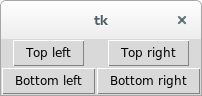
\includegraphics[width=1.75in]{img/tk_grid}
  \caption{Basic tkinter window with grid layout.}
  \label{tk_grid}
\end{figure}

As a final example, we will show a short program that uses Frames to swap
between different sets of buttons. Frames are an element that can be used
to group other elements together. We can add elements to a Frame, then add
that Frame to the window in order to display all of the elements it contains.

\lstinputlisting{lab12/frame_example.py}

Try running this code to see how it behaves. Everything here has been previously
introduced, except for the \lstinline{.grid_remove()} and \lstinline{.mainloop()}
methods. \lstinline{.grid_remove()} removes an element from its parent without
necessarily getting rid of the element.

\lstinline{.mainloop()} is a bit more
complicated. Basically, it waits for events to happen to your window and handles
them as they occur. It does not end until the window is exited. If you don't
include \lstinlinst{.mainloop()} somewhere in your program, it will simply exit
after a moment of the window popping up. Thus, a programming using tkinter
will generally set up the window and anything else it needs, then call
\lstinline{.mainloop()} and handle anything else in the commands tied to
buttons.

This is the basic flow to how using tkinter works. There are lots of other
element types you may find useful, check out the official documentation
at \url{https://docs.python.org/3/library/tkinter.html}, or the NMT-based
semi-official documentation at
\url{http://infohost.nmt.edu/tcc/help/pubs/tkinter/web/index.html}.

\pagebreak

\section{Project}
\label{sec:proj}

\begin{warningbox}{Boilerplate}
  Remember that this lab \emph{must} use the
  boilerplate syntax introduced in Lab~5.
\end{warningbox}

For this assignment, you will be creating a multiplayer game similar to the
combat system of the Pok\'emon or Final Fantasy games. You will be writing
two programs, though you are free to have them share some amount of code.
Your two main files should be named battle.py and battle\_server.py, though
you are encouraged to have more than just those two files.

Some files have been provided for you on Canvas. We recommend using them as
a starting point, though you are free to completely ignore them.

\begin{figure}[h]
  \centering
  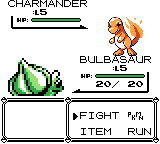
\includegraphics{img/Bulbasaur_pokemon_red}
  \caption{Pok\'emon battle screen. (from
    \href{http://en.wikipedia.org/wiki/File:Bulbasaur_pokemon_red.png}{Wikipedia})}
  \label{poke}
\end{figure}

\subsection{Game}
The game you are creating will be a two-player battle game. Each player will
have a ``party'' of monsters. At the start of the match, each player will choose
one of their three monsters to become active. Then a series of turns will occur
until one player's entire party of monsters has been defeated.

\subsubsection{Turns}
\label{subsubsec:turn}
A turn consists of each player choosing one action to perform. The possible
actions fall into two categories: switching the player's active monster or using
a move from the currently active monster.

If a player chooses to switch their active monster, they must then choose from
their current inactive and undefeated monsters. The selected monster will become
active while their current active monster will become inactive.

If a player chooses to use a move from their currently active monster, they will
then choose one of up to four moves that their monster knows.

Once both players have chosen a move for the turn, the moves will be executed.
If both players chose to switch monsters, then the order that the switches occur
does not matter. If one player chose to switch their monster while the other chose
to use a move, then the switching player's action will go first. If both players
choose to use a move, then the player whose monster has a higher Speed stat (see
Section~\ref{subsubsec:monster}) will perform its move first. The second monster
will only perform its move if it is still undefeated after the first monster
performs its move.

If at the end of a turn either or both monsters have had their Health reduced to 0
or less, then that monster has been defeated. Its user must immediately switch out
their monster for one that has not been defeated. This switch occurs before the start
of the next turn. If no undefeated monsters remain, that player has been defeated.
If both players are defeated at once, the match ends in a draw.

\subsubsection{Monsters}
\label{subsubsec:monster}  
Each monster will have a number of stats:
\begin{description}
\item[Attack] Indicates attack power of the monster. The base damage of any attack
  Move that this monster uses is modified by $$base\_damage \cdot \left(1 +
  \frac{attack}{100}\right)$$
\item[Defense] Indicates defensive strength of the monster. Any incoming damage to
  the monster is reduced by $$damage \cdot \left(1 - \frac{defense}{100}\right)$$

  A monster is not allowed to have a Defense greater than 75.
\item[Health] The maximum health that a monster has. Any time it is attacked the
  monster's current health will be reduced, thought the maximum will stay the same.
\item[Speed] Indicates the speed of the monster. Is used to determine which of the
  active monsters will use its Move first.
\item[Name] Each monster must have a name so that you can properly empathize with
  its plight.
\end{description}


In addition to these stats, each monster can have up to 4 moves, as defined in
Section~\ref{subsubsec:moves}

\subsubsection{Moves}
\label{subsubsec:moves}
A Move is an action that a monster can perform when it is active. There are four
types of Move:

\begin{description}
\item[Offensive] An offensive Move deals damage to the opponent's active monster.
  Each offensive Move has a base damage stat that helps determine how much damage it
  does, based on the two formulas in Section~\ref{subsubsec:monster}.
\item[Heal] A healing Move restores health to the monster making the Move. A healing
  Move has a stat indicating how much health it will restore. A monster cannot be
  healed above its maximum health.
\item[Buff] A Move that temporarily increases one of the active monster's stats. A buff move
  has three attributes: the stat it increases (Attack, Defense, or Speed), the
  amount it increases that stat by, and how many turns it lasts. A buff can allow a stat
  to be increased beyond the point it normally could be.
\item[Debuff] A Move that temporarily decreases one of the stats of the opponent's active
  monster. Has the same attributes as buff, but decreases instead of increases.
\end{description}

In addition to the above mentioned attributes, each move must have a name.

\subsection{Client (battle.py)}
You will need to write a client using tkinter that provides a nice user interface
to those playing the game. You should model your interface off of
Figure~\ref{poke}, though you are free to modify it as you see fit. The interface
needs to do the following:
\begin{itemize}
\item Display the name, current health, max health, attack, defense, and speed of the
  currently active monsters from both players.
\item Display information about what is happening in the game. That is, what moves each
  monster is using, what the results of those moves are, what monsters are switched for
\item Allow the user to choose between their various options each turn, as shown in
  Section~\ref{subsubsec:turn}.
\end{itemize}

In addition, your client will need to connect to your server in order to send the
actions of its player and receive the results of each turn. It will also need to
receive information about the opponent's monsters at the start of a game.

When the client is first started, it must load the information about its party
of monsters from a text file. This information must then be sent to the server upon
connection.

\subsection{Server (battle\_server.py)}
You will need to write a server that allows two clients to connect to it in order
to play the game that I really wish I had come up with a name for. This server will
carry out the majority of the game's logic and handle sending and receiving information
from the players. It will need to fulfill the following tasks:

\begin{itemize}
\item Receive information about each player's party, store that information, and
  send it to the players as necessary.
\item Wait for each player to select an action, then calculate the outcome of
  both actions.
\item Detect when one player has won and inform each player.
\item Anything else you find would be handy for the server to take care of.
\end{itemize}

You are free to use whatever protocol you wish for communicating data between the
server and the clients.



\subsection{Terms}

\begin{description}
\item[Active] The current ``fighting'' monster. Each player can only have one
  active monster at a time.
\item[Damage] The amount subtracted from a monster's current health after it is
  attacked. The full formula for damage is $$base\_damage \cdot \left(1 +
  \frac{attack}{100}\right) \cdot \left(1 - \frac{defense}{100}\right)$$
\item[Defeated] A monster that has had its health points reduced to 0. A
  defeated monster cannot be active.
\item[Monster] A mysterious creature that we are using to fight for questionably
  moral reasons. (Section~\ref{subsubsec:monster})
\end{description}

\subsection{Extra Credit}
Any or all of these can be included in your lab. If you do extra credit, include a
file called README.txt that details which extra credit opportunities you did. If
you did something extra not mentioned here, also mention it in your README.txt.
If you have any ideas for extra credit that aren't mentioned here, email
\href{mailto:rwhite00@nmt.edu}{rwhite00@nmt.edu}.

\subsubsection{Awesome Name (5 points)}
Give your game a REALLY AWESOME NAME!

\subsubsection{Status Effects (10 points)}
Implement status effects into some of your moves. That is, add some moves that have
a chance to inflict effects beyond damage and debuffs onto the enemy. For example:
\begin{description}
\item[Poison] A poisoned monster takes some amount of damage each turn for a set
  number of turns.
\item[Paralyzed] A paralyzed monster has a chance to not perform a move when it is
  selected. Additionally, a paralyzed will always move second if the other monster
  is not paralyzed.
\item[Scared] A scared monster has a chance to ignore a move command and instead
  switch itself with a random inactive undefeated monster.
\end{description}

\subsubsection{Types and Strengths/Weaknesses (15 points)}
Implement elemental types for your monsters. That is, each monster will have some
kind of alignment. Examples might be fire, water, flying, or jello. Define
(preferably in a file) weaknesses between the different types. For example,
water types might deal 150\% normal damage to fire types, while only dealing
25\% normal damage to jello types.

\begin{figure}[h]
  \centering
  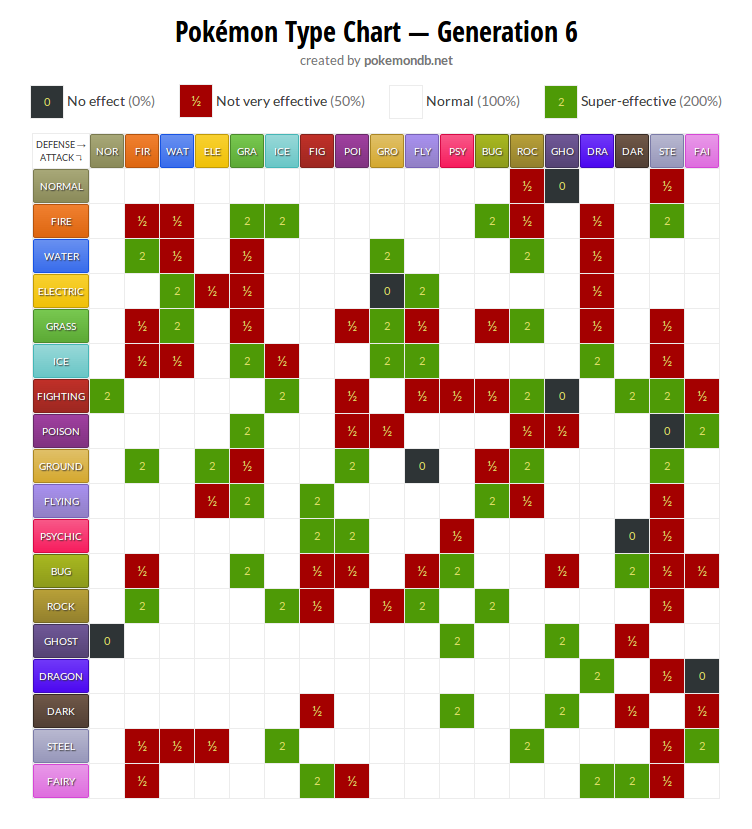
\includegraphics[width=0.5\linewidth]{img/typechart}
  \caption{Type strengths and weaknesses in Pok\'emon.}
  \label{types}
\end{figure}

\subsubsection{Validate Monster Stats (10 points)}
\label{subsubsec:valid}
Have your server validate the monsters sent in by the client to make sure they
aren't too overpowered. Make up your own rules for what determines if a monster
is valid. An example might be that the sum of all monster attributes must be less
than 250. If an invalid monster is sent to the server, send a rejection message
and either disconnect the client or request a new valid monster.

\subsubsection{Larger Party Size (10 points)}
Allow each player to have up to 6 monsters in their party instead of just 3.

\subsubsection{Monster Select (10 points)}
When the client starts and loads up a group of monsters, allow the users
to select which of the monsters they wish to use in the GUI.

\subsubsection{Monster Graphics (15 points)}
Let a monster have an associated image that is displayed on both clients.
To do this, you will need to have the client load an image, then send that
image to the server so that the server can pass it on to the other client
(remember that in a real online game
your clients won't have access to the same
files to read from, so you can't just have them both load from the same
file).

If you use images from online, make sure to cite where you got them!

\subsubsection{Randomly Generated Monsters (10 points)}
In addition to loading monsters from files, add the ability to randomly
generate a monster. You should make your randomly generated monsters have
some logic to how their stats are created so that they are not too over-
or underpowered. For examples, see Section~\ref{subsubsec:valid}.

\subsubsection{User-Created Monsters (15 points)}
In addition to loading monsters from files,
provide an interface to allow a player to create their own monsters. Let
them choose the name, stats, and whatever else youcan think of for their
party of monsters.

\subsubsection{Sound (10 points)}
Let sounds play in response to certain events. Have sound effects for
different moves, monsters being defeated, switching out monsters, and
whatever other events you want to tie sounds to.

If you use sounds from online, make sure to cite where you got them!

\subsubsection{Critical Hits (10 points)}
Allow an offensive move to have a chance to make a critical hit. For
each offensive move, give it a number from 0 to 100 indicating how
likely it is to crit. Each time the move is performed, randomly
determine -- based on that percentage -- to get a critical hit. If a
move gets a critical hit, it should do twice as much damage as normal.

Optionally, give each monster a built-in crit chance. That is, if a monster
has a built-in crit chance of $5\%$, then all of its offensive moves have
an extra $5\%$ chance to get a critical hit, even if their previous chance
was 0\%.

\subsubsection{Other Extras (?? points)}
If you have any ideas for more extra credit opportunities, email me and I
will probably add them to the lab document.



\pagebreak
\section{Submitting}

Files to submit:
\begin{itemize}
\item battle.py (Section~\ref{sec:proj})
\item battle\_server.py (Section~\ref{sec:proj})
\item Any other files created. (Section~\ref{sec:proj})
\end{itemize}

You may submit your code as either a tarball (instructions below) or as a .zip
file. Either one should contain all files used in the exercises for this lab.
The submitted file should be named either
\texttt{cse107\_firstname\_lastname\_lab12.zip} or
\texttt{cse107\_firstname\_lastname\_lab12.tar.gz} depending on which method you
used.

For Windows, use a tool you like to create a \texttt{.zip} file. The TCC
computers should have \texttt{7z} installed. For Linux, look at lab 1 for
instructions on how to create a tarball or use the ``Archive Manager'' graphical
tool.

\begin{center}
  \textbf{Upload your tarball or .zip file to Canvas.}
\end{center}

\end{document}
